\section{Results}
\label{sec:results}

\begin{table}
	\label{tab:general}
	\centering
	\caption{General measurements.}
		\begin{tabular}
		{S[table-format=1.0]
		 S[table-format=1.0]
		 S[table-format=1.2]}
		\toprule
		{$a \mathbin{/} \unit{\milli\meter}$} & 
		{$b \mathbin{/} \unit{\milli\meter}$} & 
		{$c \mathbin{/} \unit{\milli\meter}$} \\
		\midrule
		1 & 2 & 2.25 \\
		2 & 3 & 3.60 \\
		3 & 4 & 5.00 \\
		4 & 5 & 6.40 \\
 	\bottomrule
	\end{tabular}

\end{table}

\begin{table}
	\label{tab:specific}
	\centering
	\caption{Specific measurements.}
		\begin{tabular}
		{S[table-format=1.0]
		 S[table-format=1.1]}
		\toprule
		{$a \mathbin{/} \unit{\milli\meter}$} & 
		{$c \mathbin{/} \unit{\milli\meter}$} \\
		\midrule
		1 & 1.4 \\
		2 & 2.8 \\
		3 & 4.2 \\
		4 & 5.7 \\
		5 & 7.1 \\
 	\bottomrule
	\end{tabular}

\end{table}

\begin{figure}[H]
	\label{fig:plot}
	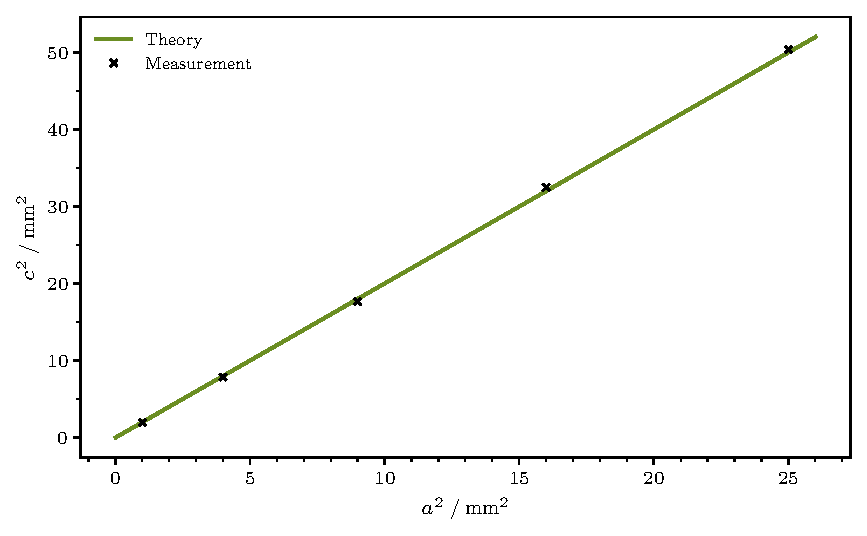
\includegraphics{build/plot.pdf}
	\caption{Measurements and theory prediction.}
\end{figure}

For $c^2 = ma^2 + n$ and using \verb+numpy.polyfit+ \cite{numpy} we find
\begin{align*}
	m = \num{2.03(0.01)} && n = \num{186.1+-2.7}
\end{align*}
as parameters.
